% paper.tex
%
% LaTeX template for creating an MNRAS paper
%
% v3.0 released 14 May 2015
% (version numbers match those of mnras.cls)
%
% Copyright (C) Royal Astronomical Society 2015
% Authors:
% Keith T. Smith (Royal Astronomical Society)

% Change log
%
% v3.0 May 2015
%    Renamed to match the new package name
%    Version number matches mnras.cls
%    A few minor tweaks to wording
% v1.0 September 2013
%    Beta testing only - never publicly released
%    First version: a simple (ish) template for creating an MNRAS paper

%%%%%%%%%%%%%%%%%%%%%%%%%%%%%%%%%%%%%%%%%%%%%%%%%%
% Basic setup. Most papers should leave these options alone.
\documentclass[a4paper,fleqn,usenatbib]{mnras}

% MNRAS is set in Times font. If you don't have this installed (most LaTeX
% installations will be fine) or prefer the old Computer Modern fonts, comment
% out the following line
\usepackage{newtxtext,newtxmath}
% Depending on your LaTeX fonts installation, you might get better results with 
% one of these:
%\usepackage{mathptmx}
%\usepackage{txfonts}

% Use vector fonts, so it zooms properly in on-screen viewing software
% Don't change these lines unless you know what you are doing
\usepackage[T1]{fontenc}
\usepackage{ae,aecompl}


%%%%% AUTHORS - PLACE YOUR OWN PACKAGES HERE %%%%%

% Only include extra packages if you really need them. Common packages are:
\usepackage{graphicx}	% Including figure files
\usepackage{amsmath}	% Advanced maths commands
\usepackage{amssymb}	% Extra maths symbols
\usepackage{mathtools}
\usepackage{hyperref}
%%%%%%%%%%%%%%%%%%%%%%%%%%%%%%%%%%%%%%%%%%%%%%%%%%

%%%%% AUTHORS - PLACE YOUR OWN COMMANDS HERE %%%%%

\newcommand{\fesc}{\ifmmode{f_{\rm esc}}\else{$f_{\rm esc}$}\fi}
\newcommand{\fescs}{\ifmmode{f_{\rm esc}^\star}\else{$f_{\rm esc}^\star$}\fi}
\newcommand{\kms}{\ifmmode{{\;\rm km~s^{-1}}}\else{km~s$^{-1}$}\fi}
\newcommand{\fgas}{\ifmmode{{f_{\rm gas}}}\else{$f_{\rm gas}$}\fi}
\newcommand{\cubecm}{\ifmmode{{\rm cm^{-3}}}\else{cm$^{-3}$}\fi}
\newcommand{\ztwo}{\ifmmode{{\rm [Z_2/H]}}\else{[Z$_2$/H]}\fi}
\newcommand{\zthree}{\ifmmode{{\rm [Z_3/H]}}\else{[Z$_3$/H]}\fi}
\newcommand{\lsim}{\lower0.3em\hbox{$\,\buildrel <\over\sim\,$}}
\newcommand{\gsim}{\lower0.3em\hbox{$\,\buildrel >\over\sim\,$}}
\newcommand{\li}{\noindent$\bullet$\quad}
\newcommand{\lli}{$\bullet$\quad}
\newcommand{\lcdm}{$\Lambda$CDM}
\newcommand{\flux}{erg s$^{-1}$ cm$^{-2}$ Hz$^{-1}$}
\newcommand{\emis}{erg s$^{-1}$ cm$^{-2}$ Hz$^{-1}$ sr$^{-1}$}
\newcommand{\sfr}{\ifmmode{\textrm{M}_\odot \,\textrm{yr}^{-1} \,\textrm{Mpc}^{-3}}\else{M$_\odot$ yr$^{-1}$ Mpc$^{-3}$}\fi}
\newcommand{\hsfr}{\ifmmode{\textrm{M}_\odot\, \textrm{yr}^{-1}}\else{M$_\odot$ yr$^{-1}$}\fi}
\newcommand{\ssfr}{Gyr$^{-1}$}
\newcommand{\arp}{$a_{\rm rp}$}
\newcommand{\agrav}{$a_{\rm grav}$}
\newcommand{\eavg}{\ifmmode{\langle E_\gamma \rangle}\else{$\langle E_\gamma \rangle$}\fi}
\newcommand{\hst}{{\it HST}}
\newcommand{\enzo}{{\sc enzo}}
\newcommand{\yt}{{\sc yt}}
\newcommand{\moray}{{\sc enzo+moray}}
\newcommand{\Ms}{\ifmmode{M_\odot}\else{$M_\odot$}\fi}
\newcommand{\vrms}{\ifmmode{v_{\rm rms}}\else{$v_{\rm rms}$}\fi}
\newcommand{\mmin}{M$_{min}$}
\newcommand{\hh}{H$_2$}
\newcommand{\Ol}{$\Omega_\Lambda$}
\newcommand{\Om}{$\Omega_M$}
\newcommand{\Ob}{$\Omega_b$}
\newcommand{\theat}{$t_{\rm{heat}}$}
\newcommand{\tcool}{$t_{\rm{cool}}$}
\newcommand{\rcool}{$r_{\rm{cool}}$}
\newcommand{\tcross}{$t_{\rm{cross}}$}
\newcommand{\tdyn}{$t_{\rm{dyn}}$}
\newcommand{\tkh}{$t_{\rm{KH}}$}
\newcommand{\tH}{$t_{\rm{H}}$}
\newcommand{\tvir}{\ifmmode{T_{\rm{vir}}}\else{$T_{\rm{vir}}$}\fi}
\newcommand{\mvir}{\ifmmode{M_{\rm{vir}}}\else{$M_{\rm{vir}}$}\fi}
\newcommand{\rvir}{\ifmmode{r_{\rm{vir}}}\else{$r_{\rm{vir}}$}\fi}
\newcommand{\rr}{$r_{200}$}
\newcommand{\lya}{Ly$\alpha$}
\newcommand{\jj}{\ifmmode{J_{21}}\else{$J_{21}$}\fi}
\newcommand{\flw}{\ifmmode{F_{LW}}\else{$F_{LW}$}\fi}
\newcommand{\kph}{\ifmmode{k_{\rm ph}}\else{$k_{\rm ph}$}\fi}
\newcommand{\tv}{$\langle T \rangle_{\rm v}$}
\newcommand{\tm}{$\langle T \rangle_{\rm m}$}
\newcommand{\msun}{{\rm\,M_\odot}} 
\newcommand{\lsun}{{\rm\,L_\odot}}
\newcommand{\zsun}{\ifmmode{\rm\,Z_\odot}\else{$\rm\,Z_\odot$}\fi}
\newcommand{\etal}{et al.\ }
\newcommand\tento[1]{$10^{#1}$}
\newcommand\step[1]{\textit{Step #1}.--}
\newcommand\halo[1]{\textit{Halo #1}.--}
\newcommand{\hi}{H {\sc i}}
\newcommand{\hii}{H {\sc ii}}
\newcommand{\hei}{He {\sc i}}
\newcommand{\heii}{He {\sc ii}}
\newcommand{\heiii}{He {\sc iii}}
\newcommand{\nhi}{\ifmmode{N_{\rm HI}}\else{$N_{\rm HI}$}\fi}
\newcommand\unit[1]{\; \textrm{#1}}
\newcommand{\pem}{\unit{s}^{-1} \unit{cMpc}^{-3}}
\newcommand{\music}{{\sc Music}}
\newcommand{\rockstar}{{\sc Rockstar}}

\newcommand{\refs}{(\textbf{Add references})}
\newcommand{\jhw}[1]{{\color{red} \bf (JHW: #1)}}


%%%%%%%%%%%%%%%%%%%%%%%%%%%%%%%%%%%%%%%%%%%%%%%%%%
%% Additions from AASTeX
%%%%%%%%%%%%%%%%%%%%%%%%%%%%%%%%%%%%%%%%%%%%%%%%%%

%\newcommand\ion[2]{#1$\;${\small\rmfamily\@Roman{#2}}\relax}
\def\eps@scaling{1.0}% 
\newcommand\epsscale[1]{\gdef\eps@scaling{#1}}% 
\newcommand\plotone[1]{% 
 \centering 
 \leavevmode 
 \includegraphics[width={\eps@scaling\columnwidth}]{#1}% 
}% 
\newcommand\plottwo[2]{% 
 \centering 
 %\leavevmode 
 %\columnwidth=.5\columnwidth 
 \includegraphics[width={\eps@scaling\columnwidth}]{#1}% 
 \hfil 
 \includegraphics[width={\eps@scaling\columnwidth}]{#2}% 
}% 

% \newcommand{\nat}{Nature}
% \newcommand{\aj}{AJ}
% \newcommand{\apj}{ApJ}
% \newcommand{\apjl}{ApJL}
% \newcommand{\apjs}{ApJS}
% \newcommand{\mnras}{MNRAS}
% \newcommand{\aap}{A\&A}
% \newcommand{\pasj}{PASJ}
% \newcommand{\pasp}{PASP}
% \newcommand{\araa}{ARA\&A}
% \newcommand{\bain}{Bull.~Astron.~Inst.~Netherlands}
% \newcommand{\memsai}{Mem.~Soc.~Astron.~Italiana}
% \newcommand{\physrep}{Physics Reports}
% \newcommand{\prd}{Phys.~Rev.~D}
% \newcommand{\jcap}{JCAP}

\hyphenation{sSFR sSFRs}

\makeatletter
\newcommand*{\rom}[1]{\expandafter\@slowromancap\romannumeral #1@}
\makeatother

% Please keep new commands to a minimum, and use \newcommand not \def to avoid
% overwriting existing commands. Example:
%\newcommand{\pcm}{\,cm$^{-2}$}	% per cm-squared

%%%%%%%%%%%%%%%%%%%%%%%%%%%%%%%%%%%%%%%%%%%%%%%%%%

%%%%%%%%%%%%%%%%%%% TITLE PAGE %%%%%%%%%%%%%%%%%%%

% Title of the paper, and the short title which is used in the headers.
% Keep the title short and informative.
\title[Where Do Pop III Stars Form?]{Where Do Population III Stars Form?}

% The list of authors, and the short list which is used in the headers.
% If you need two or more lines of authors, add an extra line using \newauthor
\author[Danielle Skinner et al.]{
Danielle Skinner,$^{1}$\thanks{E-mail: drenniks@gatech.edu}
John H. Wise,$^{1}$
\\
% List of institutions
$^{1}$Center for Relativistic Astrophysics, Georgia Institute of Technology, 
Atlanta, GA 30332, USA\\
}

% These dates will be filled out by the publisher
%\date{Accepted XXX. Received YYY; in original form ZZZ}

% Enter the current year, for the copyright statements etc.
\pubyear{2018}

% Don't change these lines
\begin{document}
\label{firstpage}
\pagerange{\pageref{firstpage}--\pageref{lastpage}}
\maketitle

% Abstract of the paper
\begin{abstract}
We perform a cosmological simulation with a comoving volume of 1 Mpc$^{3}$ to study the birthplaces of Population III stars, using the adaptive mesh refinement code \enzo{}. We investigate the distribution of host halo masses and its relationship to the Lyman-Werner background intensity.  In our sample of 697 host halos, we find that 84\% of them have masses below the Machacek et al. (2001) relation because of the inclusion of \hh{} self-shielding.  In our simulation above a redshift of 11.5, the mean halo mass is time-independent and ~10$^{5.9}$ M$_{\odot}$. Afterwards, it steadily rises above the Machacek et al. relation to a mean value of ~10$^{6.6}$ M$_{\odot}$. Most of these halos form multiple Population III stars, with a median number of four, up to a maximum of 16. We also find that a few halos do form stars below the Machacek et al. relation but in a high Lyman-Werner radiation field with values up to ~50 J$_{21}$. Our results suggest that Population III star formation may be less affected by Lyman-Werner radiation feedback than previously thought and that Population III multiple systems are common.
\end{abstract}

% Select between one and six entries from the list of approved keywords.
% Don't make up new ones.
\begin{keywords}
star formation -- methods:numerical -- cosmology
\end{keywords}

%%%%%%%%%%%%%%%%%%%%%%%%%%%%%%%%%%%%%%%%%%%%%%%%%%

%%%%%%%%%%%%%%%%% BODY OF PAPER %%%%%%%%%%%%%%%%%%
%====================================================================
\section{Introduction}
%====================================================================

The first generation of stars transformed a cold and dark universe
by illuminating and enriching up their neighborhoods with radiation
and heavy elements. The formation of these first stars is a crucial step in the cosmological evolution of the universe because the metals and feedback they deliver to their local environments are necessary for further star production and chemical enrichment. Without these initial stars, heavier metals would not have been produced, and a different universe would be observed than what is observed today. These stars are, by definition, metal-free (Population III; Pop III) and are thought to be generally massive \citep{ABN02, Bromm02_P3, Turk09, Hosokawa11, Hosokawa16, Hirano15}. A substantial fraction of these stars will generate prodigious amounts of ionizing photons and will end their lives in some form of a supernova \citep[e.g.][]{Schaerer02, Heger02}. The supernova will spread the enriched guts of the Pop III star out across its local environment, providing the area with elements the universe has not yet seen. 

Once a halo becomes chemically enriched by the death of its Pop III stars, then by definition, it can no longer form more Pop III stars. This marks the end of metal-free star formation in that pregalactic object. Understanding the mixing of metals into the environment of these halos is necessary to constrain the reach of these metals and the effects they have for future star formation. Numerical studies have shown that turbulence within halos can mix metals well down to their resolution limit \citep[][and more]{Wise08_Gal, Greif10, Smith15}. Stars will continue to form in halos, but with an increased metal abundance, these stars are now labeled as metal-enriched stars. These stars still are metal-poor, having metallicities of 10$^{-6}$ - 10$^{-2}$ of the solar abundance \citep{Chiaki16, Chiaki18, Ritter16}, have a direct chemical connection to PopIII stars, and survive until the present day \citep{Gnedin06, Tumlinson10, Griffen18, Magg18}. Understanding the formation and chemical abundance of second generation stars can provide more evidence and insight for the earlier generation of Pop III stars.

Given the paradigm of hierarchical structure formation, halos grow through smooth accretion and successive mergers of smaller halos. But in which halos do these first generations of stars form? Their formation rates and locations are important to constrain because they influence the very beginnings of galaxy formation and cosmic reionization. Learning about their host halos can also guide future telescopic surveys to observe Pop III galaxies which may lead to their direct observational evidence. Previous studies have investigated the possibility of finding Pop III systems. For example, \citet{Trenti09} found that metal-free halos may still be able to form at $z \approx$ 6, which offer the best chance at observing such primordial systems. They find that, given a certain rate of Pop III supernova per year, large sky surveys, such as the Large Synoptic Survey Telescope (LSST), should be able to detect the very luminous supernova. \citet{Trenti09} determine that unless the metal-free systems are particularly efficient at forming Pop III stars (star formation efficiencies > 10$^{-2}$), the upcoming James Webb Space Telescope (JWST) will not be able to detect such systems.

Various semi-analytic investigations have been conducted to learn more about the halo collapse criterion, and thus, which halos can host Pop III stars. \citet{Tegmark97} discovered that halos can have a strongly redshift dependent, minimum baryonic mass of 10$^{6}$ M$_{\odot}$ at $z \approx$ 15. In particular, they derive an analytic expression for the fraction of \hh{} needed in a halo for efficient cooling, and determine which  halos can cool in a Hubble time. \citet{Visbal18} devised a semi-analytic model for the formation of Pop III stars and the transition to metal-enriched stars. They find that varying the Pop III star formation efficiency, the time from a Pop III supernova to metal-enriched star formation, the external enrichment of the halo, and the ionizing escape fraction, leads to large differences in the star formation history of Pop III and metal-enriched stars. This method is useful for exploring the wide parameter space of star formation in the early universe, and could lead to further constraints in the future. 

Without metals and dust to facilitate efficient radiative cooling, Pop III stars rely on \hh{} formation to cool the gas. These molecules are however fragile to dissociation from Lyman-Werner (LW) radiation in the energy range 11.2--13.6~eV, through the Solomon process \citep{Field66, Stecher67}. This is a two-step process through which H$_{2}$ is excited to a higher state, H$_{2}^{\ast}$, via absorption of a LW photon:
\begin{equation} \label{Solomon1}
	H_{2} + \gamma \rightarrow  H_{2}^{\ast}
\end{equation}
This excited state then has a probability of dissociating into two hydrogen atoms:
\begin{equation} \label{Solomon2}
	H_{2}^{\ast} \rightarrow H + H
\end{equation}

Diffuse gas is optically thin to LW radiation, thus a background builds over time and can suppress \hh{} formation, delaying Pop III star formation. Furthermore, nearby sources of LW radiation can boost the intensity above the background value which facilitates further \hh{} dissociation in minihalos. This process can be counteracted with a sufficient amount of \hh{} already present within a halo, via \hh{} self-shielding. Halos with an \hh{} column density of N$_{\rm H2}$ $\geq$ 10$^{14}$ cm$^{-2}$ can suppress the photodissociation of \hh{} by LW photons \citep{Draine96}, giving the halo a chance to form Pop III stars. Other sources of the suppression of Pop III star formation are streaming baryonic velocities \citep{Tselia11, Greif11_Delay, Naoz12,OLeary12}, arising from recombination, and dynamical heating, occurring during the virialization of halos \citep{Yoshida03, Fernandez14}. 

Previous work have mainly investigated and established the lower limit for a halo to host Pop III stars, or for a halo to collapse. However, subsequent simulations have shown that they do not necessarily form at this minimum due to the aforementioned physical processes playing a role. \citet{Mebane18} used a semi-analytic model of early star formation and found that the LW background coming from the rapidly increasing supply of Pop III stars becomes responsible for suppressing Pop III star formation. \citet{Griffen18} also find that the LW background can significantly suppress the amount of potential sites for Pop III star formation. 

Numerical simulations have also been employed to investigate collapse thresholds and Pop III star formation. \citet[hereafter M01]{Machacek01} found similar results to those mentioned previously, in that the LW feedback can suppress the collapse of small mass halos. They derive a simple analytic expression for the mass threshold of halos given a particular LW flux:
\begin{equation} \label{mthresh}
	M_{\rm TH} ( M_{\odot} ) = 1.25 \times 10^{5} + 8.7  \times 10^{5} \left( \frac{4 \pi J_{\rm LW}}{10^{-21}} \right)^{.47}
\end{equation}
We will compare our results with this relation in future sections. \citet{Yoshida03} also finds that cooling is inefficient in halos with a LW background > 0.01 J$_{\rm 21}$, although with sufficient \hh{} shielding, halos are able to cool in the given LW background radiation. In fact, \citet{Wise07_UVB} found that central shocks drive \hh{} formation, allowing the halo to cool in a LW background intensity of 1 J$_{21}$. They find that \hh{} cooling is always a dominant process, even in large LW background fluxes. Assisting this result, \citet{OShea08} find that Pop III star formation can occur in relatively high LW backgrounds, implying that the LW background may not be a complete indicator of whether or not Pop III stars will form in a given halo.    

In this paper, we focus on the distribution of host halo masses, not just the minimum, and its dependence on redshift and the LW background, augmenting results from prior work. We aim to provide further insight into the host halos of Pop III stars. In \S 2 the methods of the simulation, implementation of star formation, feedback, and \hh{} self-shielding are described. In \S 3 we present the results of our analysis. In \S 4 we discuss the results in more detail and compare with previous work. In \S 5 we conclude our discussion with a summary of our results and the implications therein.

%====================================================================
\section{Methods}
%====================================================================
\subsection{Simulation setup}
%====================================================================
We run and analyze a cosmological simulation with the adaptive mesh refinement (AMR) code \enzo{} \citep{Enzo} and the toolkit \yt{} \citep{yt_full_paper}. \enzo{} uses an N-body adaptive particle-mesh solver \citep{Efstathiou85, Couchman91, BryanNorman1997} to follow the dark matter (DM) dynamics. We use the nine-species (\hi, \hii, \hei, \heii, \heiii, e$^{-}$, H$_{2}$, H$_{2}^{+}$, H$^{-}$) non-equilibrium chemistry model \citep{Abel97, Anninos97}. This simulation is similar to the RP simulation in \citet[hereafter W12]{Wise12_RP}, but with updated cosmological and Pop III parameters, and the inclusion of \hh{} shielding.

We simulate a 1 Mpc$^{3}$ comoving box with a 256$^{3}$ base grid 
resolution and a dark matter paticle mass of 2000 M$_{\odot}$. It has a maximum refinement level of 12 which provides a maximal comoving resolution of $\sim$1 pc. The simulation is 
initialized with \music{} \citep{Hahn11_MUSIC} at $z$ = 130 and uses the cosmological parameters from the Planck collaboration best fit 
\citet{Planck13_Cosmo}: $\Omega_{M}$ = 0.3175, $\Omega_{\Lambda}$ = 
0.6825, $\Omega_{DM}$ = 0.2685, and h = 0.6711, with the variables 
having their usual definitions. The simulation is run until $z$ = 9.32, when it becomes too computationally expensive to continue. At this point, 20\% of the volume is ionized. We output 918 datasets,  roughly 0.5 Myr apart. In this paper, we focus only on outputs where Pop III stars have just formed, from $z$ = 27.23 to 9.39. 

A time-dependent LW optically thin radiation background is applied in the simulation. This was fit in W12 (see their Eq. 16) and is consistent with the values in \citet{Trenti09_SFR}. The background evolution of the specific intensity takes the following form:
\begin{equation} \label{LWbg}
	\log_{10}(J_{\rm LW}/J_{21}) = A + Bz - Cz^{2} + Dz^{3} - Ez^{4}
\end{equation}
where $(A, B, C, D, E)$ = $(-2.567, 0.4562, - 0.02680, 5.882 \times 10^{-4}, - 5.056 \times 10^{-6})$ and J$_{21}$ is a specific intensity of 10$^{-21}$ erg s$^{-1}$ cm$^{-2}$ Hz$^{-1}$ sr$^{-1}$. 

We use adaptive ray tracing \citep{Abel02_RT, Wise11_Moray} to evolve the radiation field. Centered on each metal-enriched and Pop III star, we model the \hh{} dissociating radiation field with an optically thin, inverse square profile. These LW sources are added on top of the background intensity described above.
%====================================================================
\subsection{Star formation}
%====================================================================
In this section, we will discuss how we implement Pop III and metal-enriched star formation. We do not consider the formation and feedback from stellar remnants or asymptotic giant branch (AGB) stars. For further details, we refer the reader to W12. 

%====================================================================
\subsubsection{Pop III Star Formation and Feedback }
%====================================================================
The utilized Pop III star formation model is the same as in \citet{Wise08_Gal}. Each star particle represents a single star, and is formed in a cell when the following criteria are met: 
\begin{enumerate}
	\item a metallicity Z $\leq$ 5 $\times$ 10$^{-6}$ Z$_{\odot}$

	\item a gas number density n > 10$^{6}$ cm$^{-3}$

	\item converging gas flow, $\nabla \cdot \mathbf{v_{gas}}$ < 0 

	\item molecular hydrogen fraction, f$_{\rm H2}$ > 10$^{-3}$
\end{enumerate}

If within 1 pc, multiple cells meet this criteria, then a single Pop III star forms at the center of mass of these cells. The mass of the Pop III star is randomly sampled from an initial mass function (IMF) of the form:
\begin{equation} \label{IMF}
	f(\log M)dM = M^{-1.3} \exp \left[-\left( \frac{M_{\rm char}}{M}\right)^{1.6} \right]dM
\end{equation}
where M$_{\rm char}$ = 20 M$_{\odot}$ \citep{Hirano17}. This characteristic mass is different from W12 \citep{Hirano17}. This results in an exponential cutoff before M$_{\rm char}$ and a power-law IMF after. Once the cell meets the above criteria and the stellar mass is chosen, an equal amount of gas is removed from the grid in a sphere which contains twice the stellar mass that is centered on the new star particle. The new Pop III star then gains the mass-weighted velocity of the gas contained within that sphere.  

We use the mass-dependent hydrogen ionizing and LW luminosities and lifetimes from \citet{Schaerer02} and a mass-independent photon energy of E$_{\rm ph}$ = 29.6 eV, which is appropriate for the nearly mass-independent surface temperature of Pop III stars, at 10$^{5}$ K. A Type II supernova results if the Pop III star dies with a mass between 11 $\leq$ M$_{\star}$/M$_{\odot}$ $\leq$ 40. A pair instability supernova (PISNe) results if the star dies with a mass between 140 $\leq$ M$_{\star}$/M$_{\odot}$ $\leq$ 260. Outside of these mass ranges, the Pop III star dies as a black hole. In this simulation, no black hole physics are implemented, so the Pop III star simply turns into a collisionless particle. When 11 $\leq$ M$_{\star}$/M$_{\odot}$ < 20, the star dies as a normal Type II supernova with an energy of 10$^{51}$ erg. From 20 $\leq$ M$_{\star}$/M$_{\odot}$ $\leq$ 40, the star dies as a hypernova with energies taken from \citet{Nomoto06}. The PISNe have explosion energies from \citet{2002ApJ...567..532H}, of which the analytic function fit to their models can be seen in Eq. 12 of W12. 

%====================================================================
\subsubsection{Pop II  Star Formation and Feedback}
%====================================================================
The Pop II star formation model is the same as \citet{Wise09}, which is equivalent to the above criteria for Pop III star formation but without the molecular hydrogen fraction requirement, and with a metallicity greater than the above value. Star formation is only allowed for gas with temperatures $T$ < 1000 K, to ensure that the volume is cold and collapsing. Contrary to Pop III stars representing single star particles, metal-enriched star particles are modelled as clusters of stars. We enforce a minimum mass of M$_{min}$ = 1000 M$_{\odot}$ for these star particles. 

The lifetime of these particles is 20 Myr, during which they radiate 6000 hydrogen ionising photons per stellar baryon, or 1.13 $\times$ 10$^{46}$ photons s$^{-1}$ M$_{\odot}^{-1}$, which is appropriate for a Salpeter IMF. Their spectra are approximated with a monochromatic spectrum with an energy of 21.6 eV at a constant luminosity. After living for 4 Myr, the stars begin to return supernova energies of 6.8 $\times$ 10$^{48}$ erg s$^{-1}$ M$_{\odot}^{-1}$ back to their surroundings.

%====================================================================
\subsection{\hh{} Self-Shielding}
%====================================================================
We use the Sobolev-like approximation from \citet{Wolcott11} to model \hh{} self-shielding. To determine the \hh{} shielding factor, the column density of \hh{} needs to be calculated:
\begin{equation} \label{Nh2}
	N_{\rm H2} = n_{\rm H2}L_{\rm char} \ ,
\end{equation}
where n$_{\rm H2}$ is the number density of \hh{} and L$_{\rm char}$ is a characteristic length over which n$_{\rm H2}$ is assumed to be constant. The method employed in this simulation is to define the characteristic length as:
\begin{equation} \label{Lchar}
	L_{\rm char} = \frac{\rho}{|\nabla \rho|}
\end{equation}
This Sobolev-like method determines the length over which gas with density $\rho$ is diminished. They found that the most accurate, non-ray tracing, method is to use a single Sobolev-like length determined from the mean Sobolev-like length over all Cartesian directions. 

Upon numerically calculating the shielding factor of \hh{} for simulated protogalaxies, Wolcott-Green et al. determine that a slight adjustment to the shielding factor from \citet{Draine96} is sufficient to account for inaccuracies at higher temperatures. The implemented shielding factor is then (see Eq. 10 in \citet{Wolcott11}):
\begin{equation} \label{shield}
	\begin{multlined}
	f_{\rm sh}(N_{\rm H2}, T) = \frac{0.965}{(1+x/b_{5})^{1.1}} + \frac{0.035}{(1+x)^{0.5}}  \times \\ \exp [-8.5 \times 10^{-4} (1+x)^{0.5}]
	\end{multlined}
\end{equation}
Here, x $\equiv$ N$_{H_{2}}$/5 $\times$ 10$^{14}$ cm$^{-2}$, b$_{5}$ $\equiv$ b/10$^{5}$ cm s$^{-1}$, and $b$ is the Doppler broadening parameter.


%====================================================================
\section{Results}
%====================================================================
In this section, we will present the distribution of host halo masses of Pop III stars, the relation between the mass distribution and the LW background radiation, and the distribution of various Pop III properties.

%====================================================================
\subsection{Population III host halo masses}
%====================================================================
To ensure that our box is representative of a typical piece of the universe, Figure \ref{fig:hmf} shows the numerical halo mass function along with the analytic Sheth-Tormen mass function at $z$ = 9.3. The analytic function closely matches our simulation until the mass resolution of our simulation is unable to resolve below 10$^{5}$ M$_{\odot}$ halos that contain $\approx$50 particles. 

\begin{figure}
	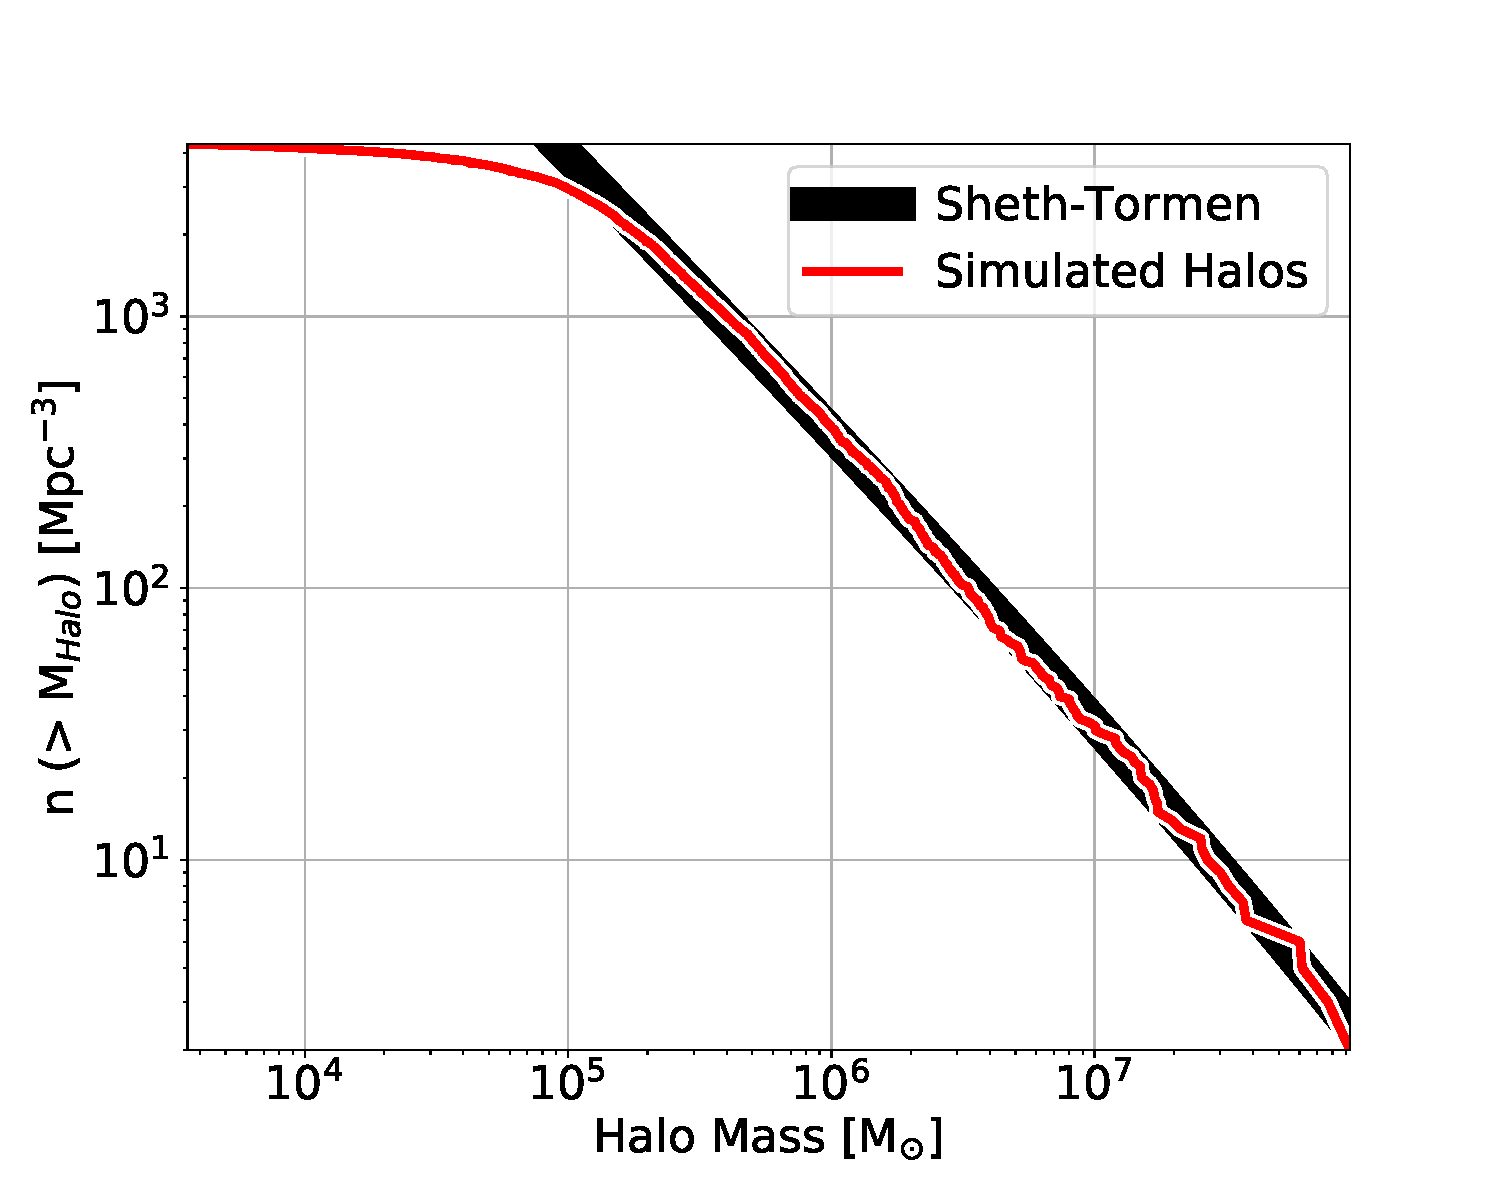
\includegraphics[width=\columnwidth]{images/hmf.pdf}
    \caption{Halo mass function of the last output of the simulation at $z$ = 9.3. The thick, black line is the analytic Sheth-Tormen mass function. The distribution of halo masses matches well with Sheth-Tormen until about 10$^{5}$ M$_{\odot}$.}
    \label{fig:hmf}
\end{figure}

As mentioned previously, Pop III stars form in our simulation only between 27.23 $\geq z \geq$ 9.39. During this time frame, a total of 697 Pop III stars form. The corresponding star formation rate density can be seen in Figure \ref{fig:pop3_SFR_bar}. Pop III star formation peaks at a redshift of 20 and slowly decreases. The star formation rate density does not fall to zero at the end of the simulation, since Pop III stars were still being produced when the simulation was cut off. To determine the host halos of new Pop III stars, we use the halo finding code, \rockstar{} \citep{rockstar}. The mass determined by \rockstar{} is the dark matter mass, so to determine the total mass of the halos, we multiply the masses by $\Omega_{\rm M}$/$\Omega_{\rm DM}$. The total mass is subsequently used in our analysis. We also take the center and virial radius from the \rockstar{} halo catalog. A small percentage of Pop III stars do not form in a halo identified by \rockstar{}. Assuming that Pop III stars must form in collapsed halos, we calculate the virial mass and radius of a halo centered on the Pop III star directly from the simulation data. We calculate the LW intensity impinging on each halo by summing up the contribution coming from each radiating star particle outside the virial radius of the host halo. This is then added to the constant LW background implemented in the simulation (Eq. \ref{LWbg}). 

\begin{figure}
	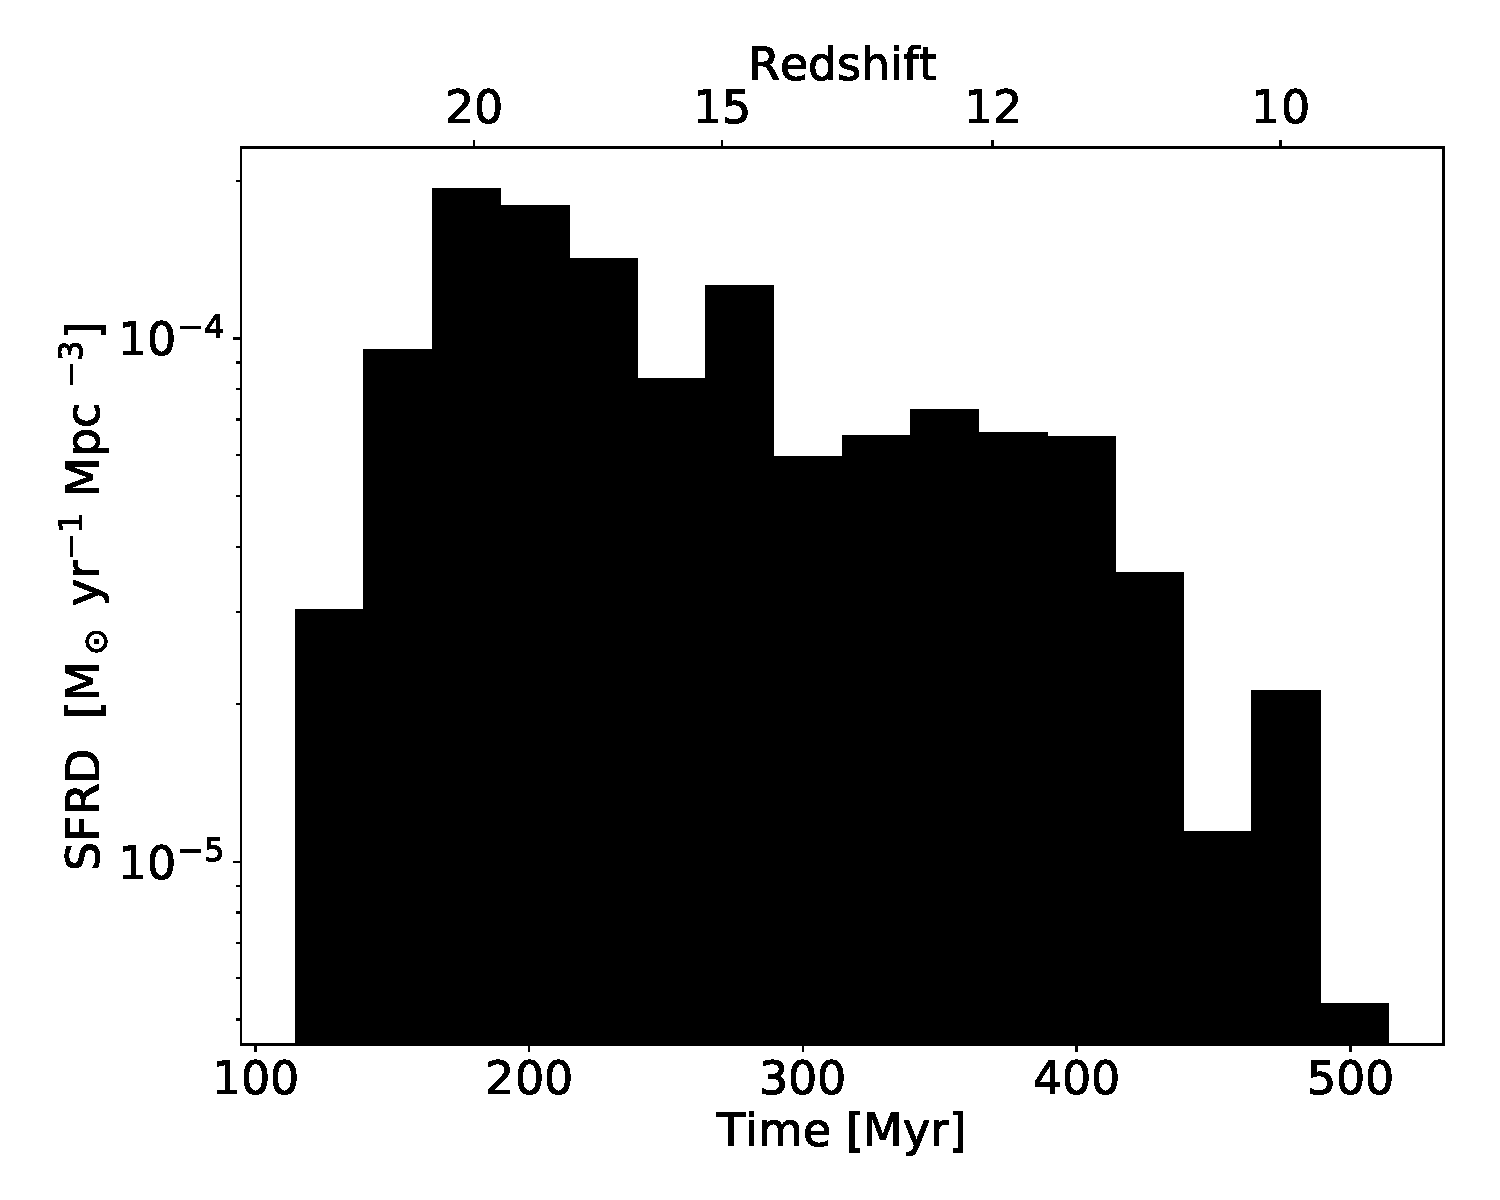
\includegraphics[width=\columnwidth]{images/pop3_SFR_bar.pdf}
    \caption{The star formation rate density of Pop III stars. It peaks at a redshift of 20, and slowly falls off.}
    \label{fig:pop3_SFR_bar}
\end{figure}

In redshift bins of $\Delta z$ = 1, the mean halo mass hosting Pop III stars is determined, and plotted against the redshift bins in Figure \ref{fig:mean_mass}. The M01 relation (Equation \ref{mthresh}) is plotted using the LW background intensity in Eq. \ref{LWbg}. Notably, the mean halo mass falls well below the relation, at 10$^{5.9}$ M$_{\odot}$ until $z$ = 11.5, at which point, the mean halo mass rises to 10$^{6.6}$ M$_{\odot}$. The large discrepancy between our data and the mass threshold from M01 is indicative of the \hh{} shielding which is included in our simulation. \hh{} shielding allows for halos to form at much lower masses, and therefore, Pop III stars are forming in these halos at earlier times. In the M01 analysis, \hh{} shielding is neglected in their calculations for a variety of reasons, including the Doppler broadening of LW bands and large column densities of \hh{} only beginning to form at late times. Interestingly, a full radiative transfer simulation, such as ours, does not produce identical results as M01 predicts. As can be seen by the red solid line in \ref{fig:mean_mass}, nearly 100\% of the halos hosting Pop III stars fall below the M01 relation, until around a redshift of 15, at which point, the mean halo mass begins to rise above the relation. Throughout the literature, there appears to be a consensus that \hh{} self-shielding will help smaller mass halos collapse in the presence of a LW background radiation \citep[E.g.][]{Yoshida03, Ricotti01, Glover01, Hartwig15}.

\begin{figure}
	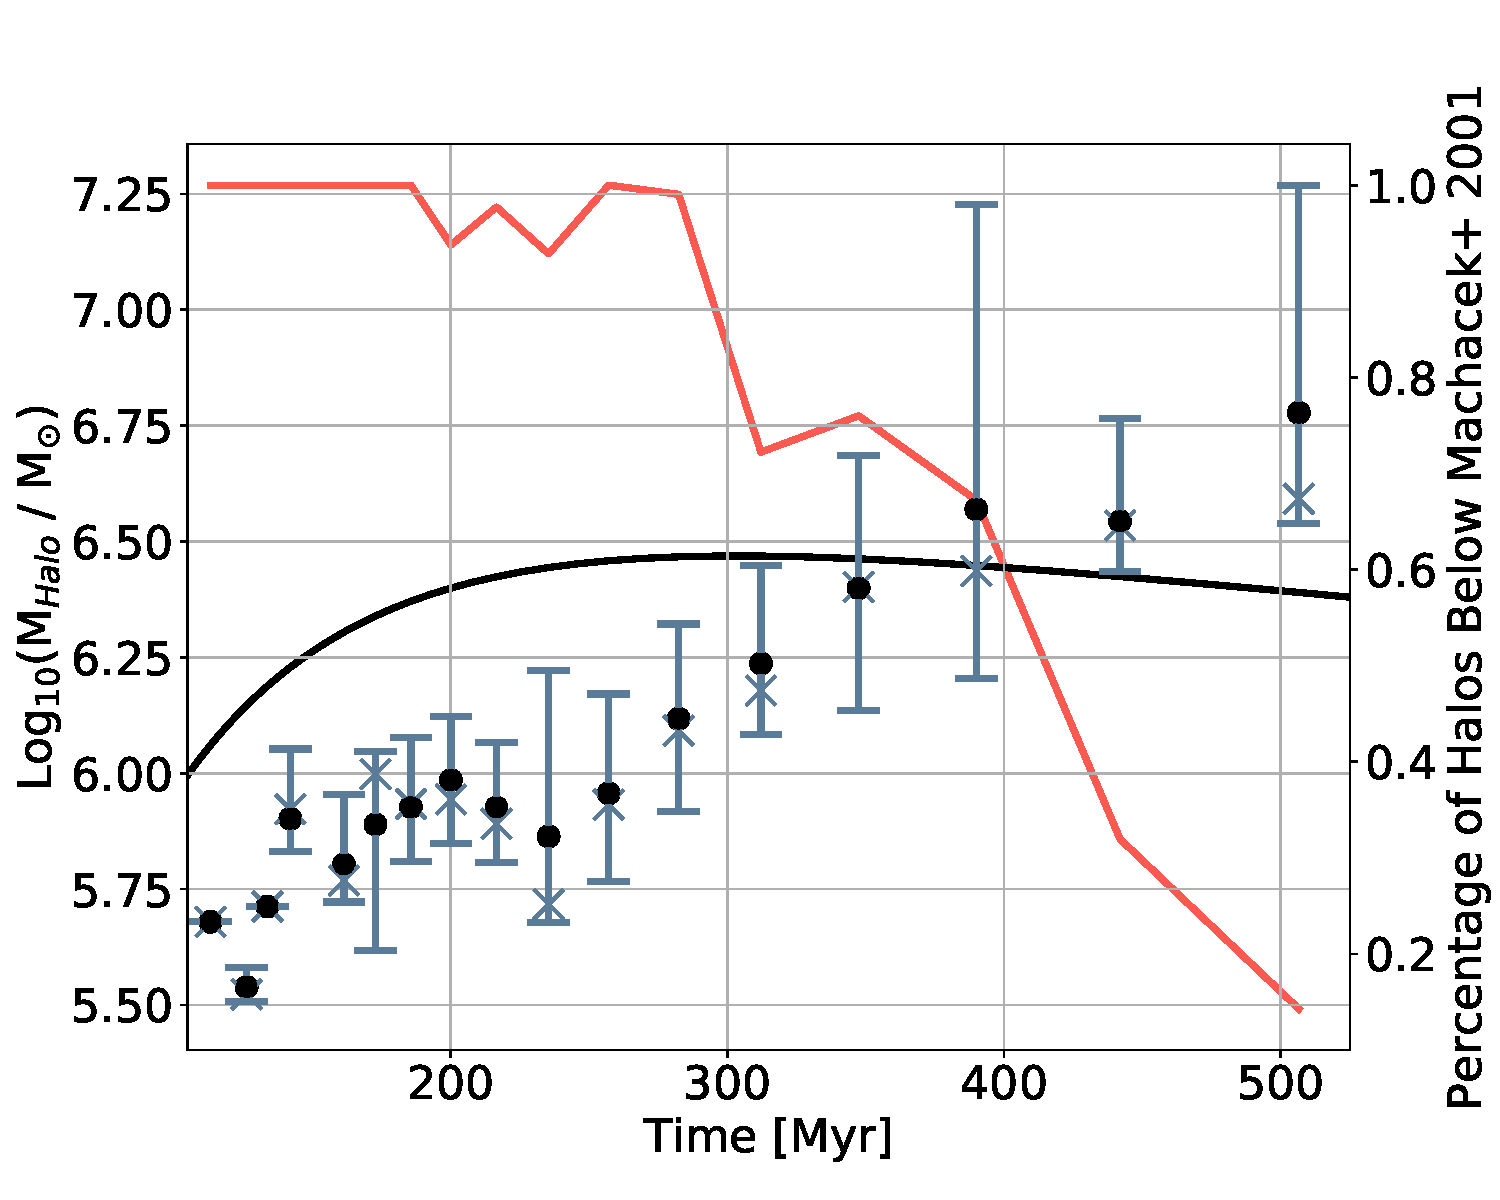
\includegraphics[width=\columnwidth]{images/mean_mass_errorb_fix.pdf}
    \caption{For halos hosting new Pop III stars, the mean halo mass for redshift bins of $\Delta z$ = 1 is plotted along the left hand side versus redshift. The black scatter points indicate the mean halo mass for that redshift bin and the x indicate the median halo mass. The error bars indicate the 15.1\% and 84.1\% percentiles. Plotted along the right hand side is the percentage of halos that fall below the M01 mass threshold, also plotted along redshift. The M01 mass threshold (Eq. \ref{mthresh}), is plotted for the constant LW background in Eq. \ref{LWbg}. Almost all halos fall below the M01 relation, until $z$ = 11.5, when the mean halo mass rises above the relation.}
    \label{fig:mean_mass}
\end{figure}

The LW background intensity is plotted versus the host halo mass for each Pop III halo in our dataset in Figure \ref{fig:jlw_mass_machacek}. Each point is colored by the redshift where the Pop III star forms and the mass threshold from M01 (Eq. \ref{mthresh}) for the given LW background (Eq. \ref{LWbg}) is also plotted. We see that almost all halos form below the M01 threshold. There are also a few halos that form Pop III stars in very high J$_{\rm LW}$, below the relation. This situation arises when there are multiple Pop III stars forming at about the same time, within $\approx$ 90 pc of each other. Star formation can occur in a neighboring halo of a Pop III star whose LW radation does not have ample time to photodissociate enough \hh{} to completely suppress star formation. The high J$_{\rm LW}$ is generally an indicator that the halos will likely have their star formation suppressed, but in cases where Pop III star formation occurs synchronically, star formation will not be suppressed, so long as they are a suitable distance away from each other. As there are only a few data points in this region, this situation is rare. It should be noted that there may be duplicate halos within this plot, since halos are allowed to form multiple Pop III stars if the conditions are sufficient and each point represents an instance of Pop III formation. The grouped points in the higher end of J$_{\rm LW}$ are representative of such halos. We find that a total of 84\% of the halos forming Pop III stars lie below the M01 mass threshold over the entire simulation redshift range. 

%====================================================================
\subsection{Multiple stellar systems}
%====================================================================

We now inspect the number of Pop III stars and the total mass of Pop III stars per halo. Figure \ref{fig:totnump3_halomass_sidehist} shows the number of Pop III stars per halo for a given halo mass. The histogram of the number of Pop III stars for all masses is projected on the right hand side. We find that a median number of four Pop III stars form per halo, with a maximum of 16 Pop III stars forming per halo. Since we did not restrict the number of Pop III stars that can form in a halo, we find that the conditions are often sufficient for multiple Pop III stars to form in a single halo. Out of the halos forming Pop III stars, only 16\% of them form single PopIII stars, whereas 54\% form between two and five Pop III stars. Figure \ref{fig:totp3mass_halomass_sidehist} shows the total mass of Pop III stars per halo for a given halo mass, where the histogram of the total Pop III mass for all halos is projected on the right hand side. Lines of constant star formation efficiency are overplotted. We find that most of our Pop III stars are forming between 10$^{-4}$ < f$_\star$ < 10$^{-3}$. The mean total mass of Pop III stars for all halos is 195 M$_{\odot}$.  


\begin{figure}
	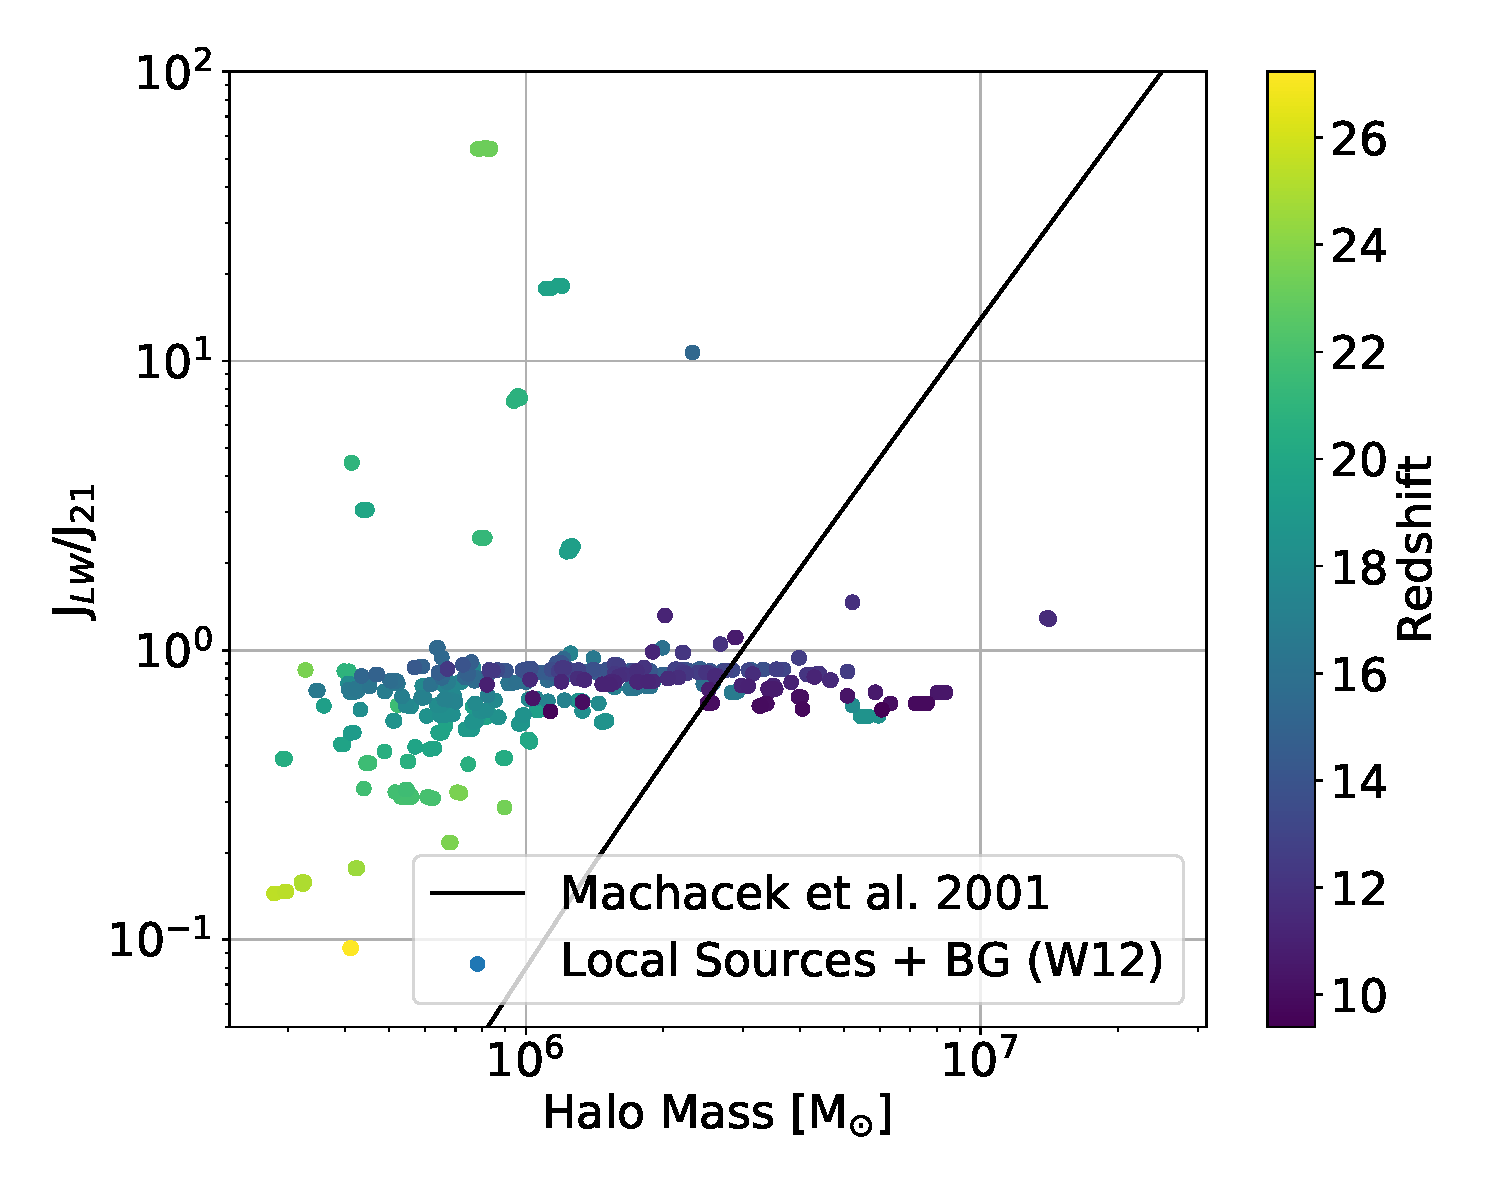
\includegraphics[width=\columnwidth]{images/jlw_mass_machacek_total.pdf}
    \caption{The average LW background for host halos of new Pop III stars is plotted versus the host halo mass, colored by redshift. The Machacek et al. relation is plotted given the background LW in Eq. \ref{LWbg}. Almost all halos fall below the relation, across a range of redshifts. A few halos (or possibly a single halo) allow Pop III stars to form at a low halo mass in a very high LW background. There are a few halos that have Pop III stars forming at later times and at high halo masses.}
    \label{fig:jlw_mass_machacek}{}
\end{figure}

\begin{figure}
	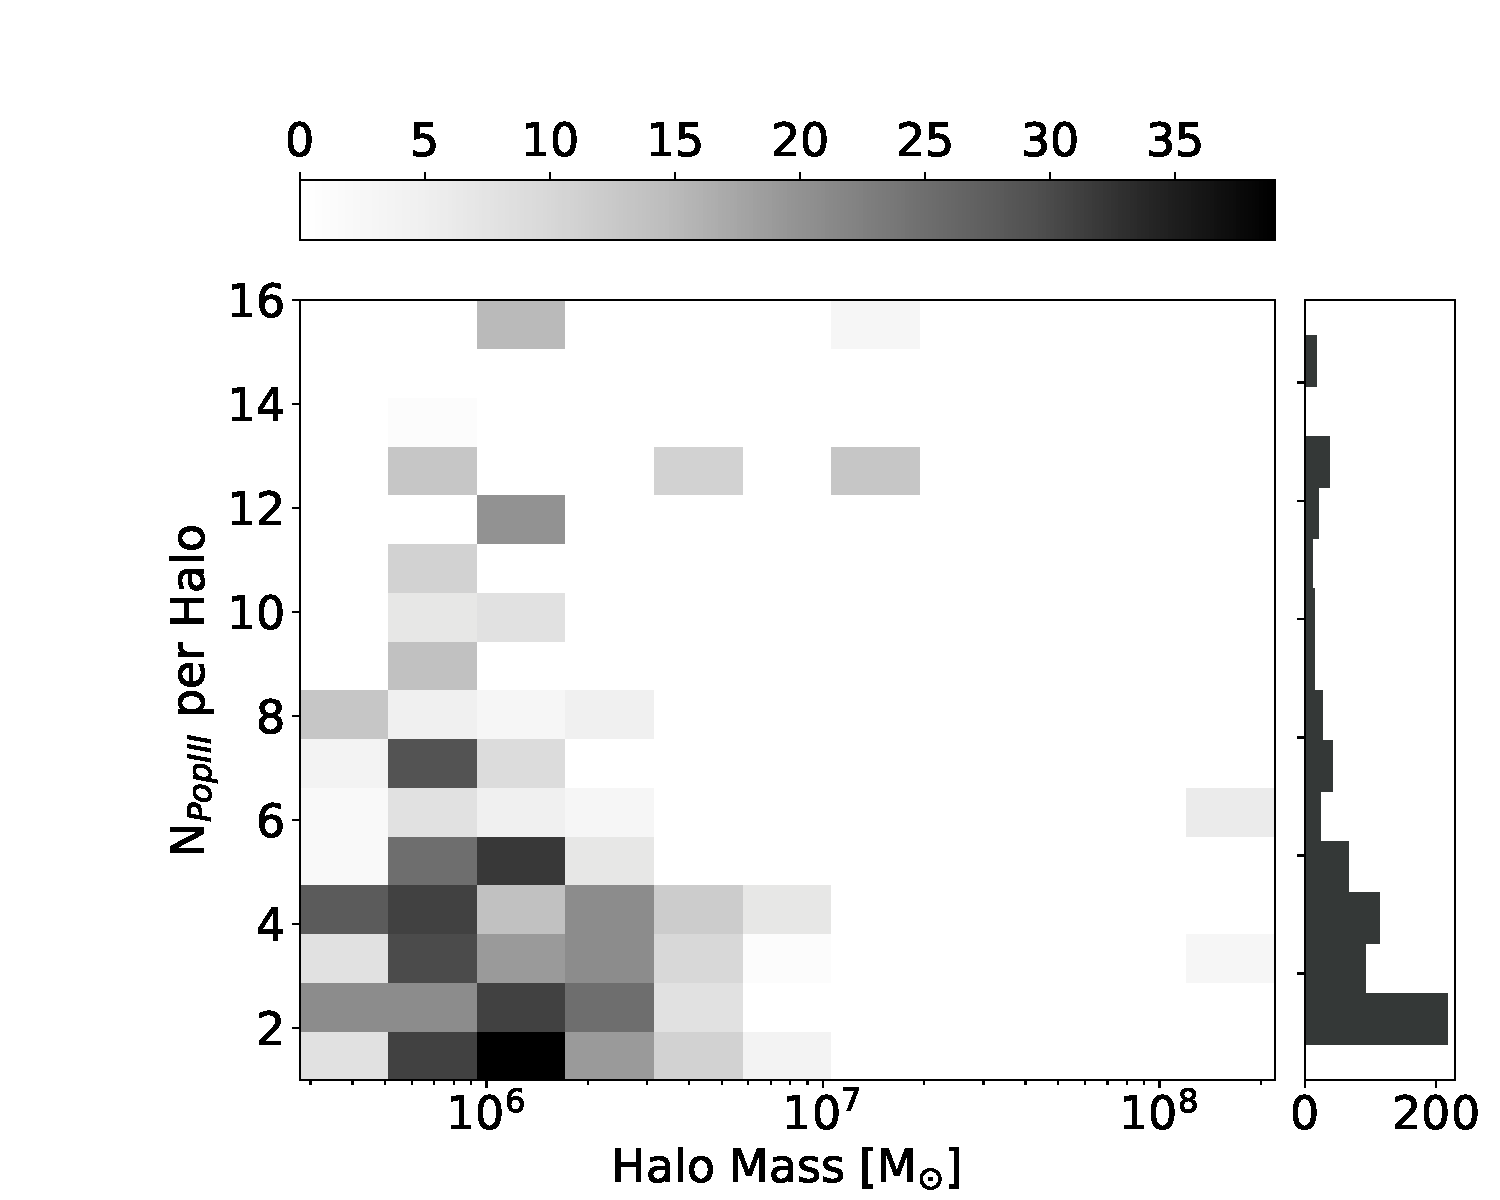
\includegraphics[width=\columnwidth]{images/totnump3_halomass_sidehist.pdf}
    \caption{Total number of Pop III stars in halos hosting new Pop III stars versus halo mass. A median number of four Pop III stars form in a single halo, with some forming as many as 16 Pop III stars.}
    \label{fig:totnump3_halomass_sidehist}
\end{figure}

\begin{figure}
	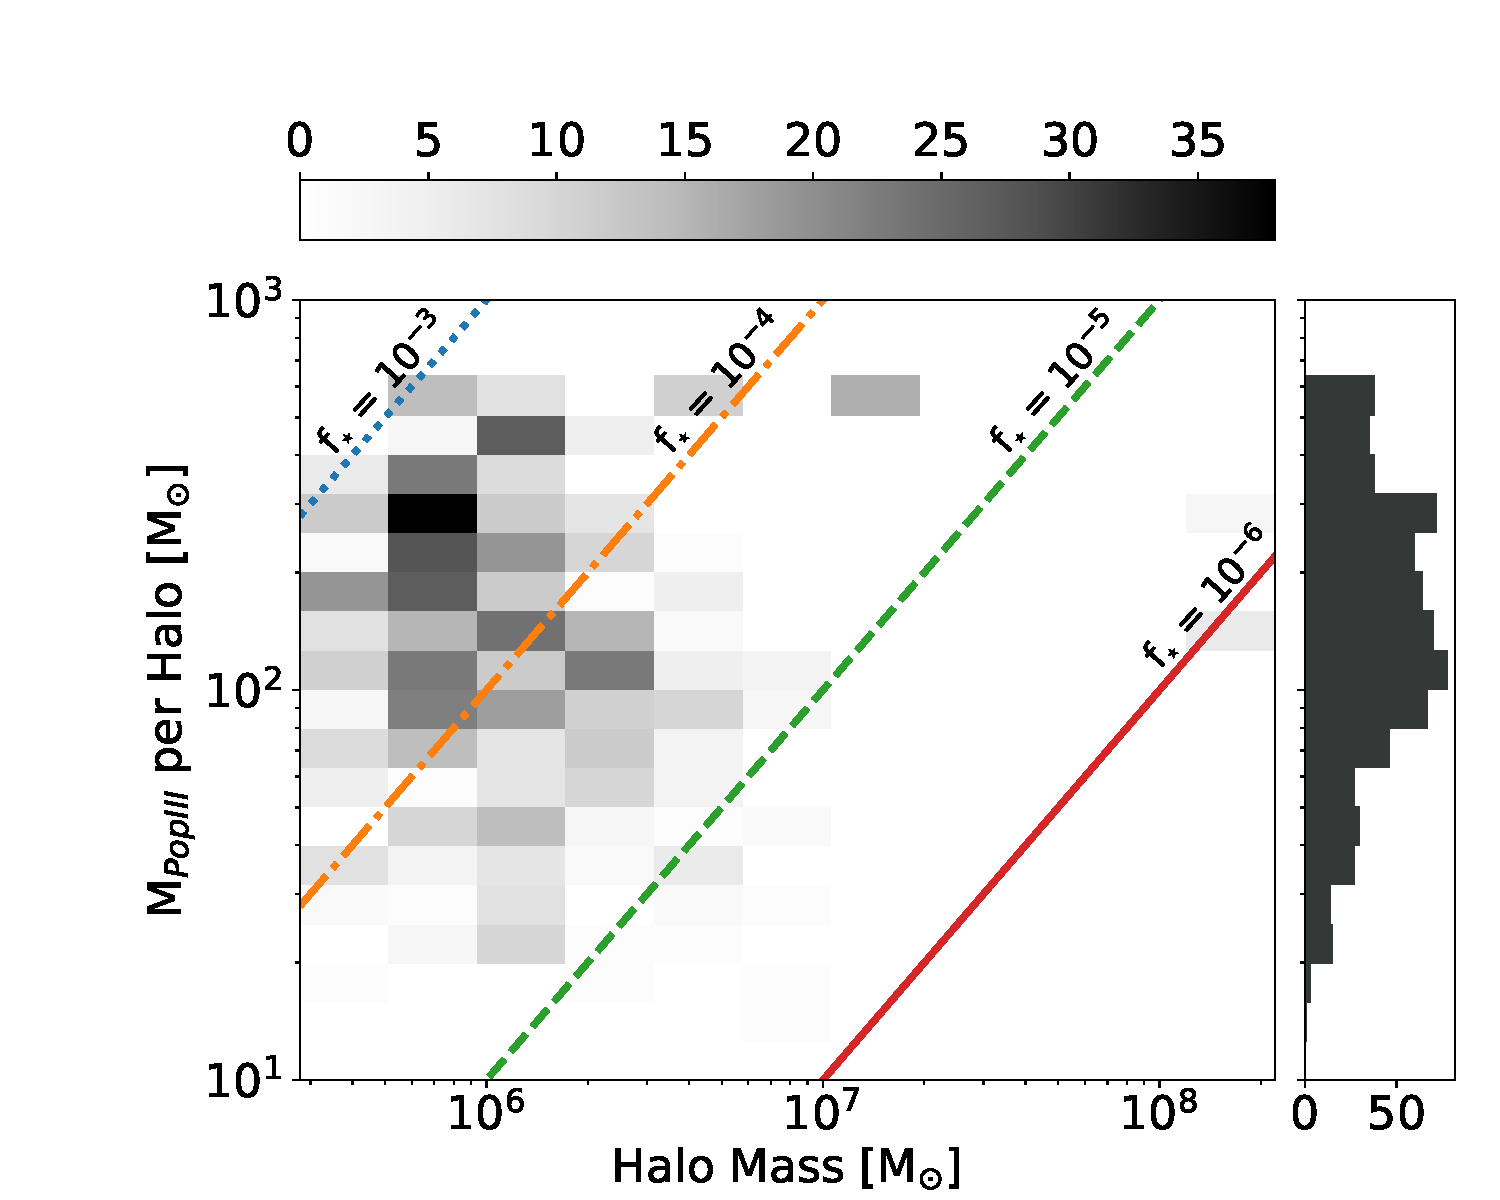
\includegraphics[width=\columnwidth]{images/totp3mass_halomass_sidehist.pdf}
    \caption{Total mass of Pop III stars in halos hosting new Pop III stars versus halo mass. Lines of constant star formation efficiencies are overplotted. Most halos form Pop III stars at efficiencies between 10$^{-3}$ and 10$^{-4}$.}
    \label{fig:totp3mass_halomass_sidehist}
\end{figure}

%====================================================================
\section{Discussion}
%====================================================================

%====================================================================
\subsection{Variations in the halo masses at collapse}
%====================================================================
The collapse of gas that goes on to form Pop III stars occurs in a wide range of host halo masses across time. There are three main reasons why the host halo masses may vary significantly. First, a generation of metal-free stars can form if their progenitors had only formed stars that did not go supernova. This prevents metals from enriching the environment which would stop metal-free star formation and begin metal-enriched star formation. Second, dynamical heating from mergers and accretion can heat the gas within halos and prevent \hh{} regions from cooling. This would delay star formation in halos with a large dynamic range at early times (not sure if dynamic range is the right way to say this) \citep{Yoshida03}. Finally, temporal fluctuations in the local Lyman-Werner radiation field can greatly affect the amount of \hh{} within a halo and thus, how efficiently the halo can cool. While this may only be a small affect in some halos where the local Lyman-Werner radiation is relatively low, Pop III star formation may be significantly delayed or completely prevented in halos that are close to active Pop III star formation sites. The combination of these three processes will determine which halos will be able to form Pop III stars, and thus results in a wide range of host halo masses. 


%====================================================================
\subsection{Comparison to previous work}
%====================================================================

\li Semi-analytic papers: \citep{Tegmark97, Trenti09, Visbal18,
  Mebane18, Griffen18}

\noindent\textbf{JHW summary:} In all of these papers, we shouldn't be focusing on the redshift dependence because that relies on the galaxy/star formation model that has large uncertainties.  We should focus on the relationship between the LW background intensity and the halo masses.  This is the best thing to do because our cosmological volume is small and cannot capture the cosmic variance.  The Tegmark+ result is the absolute lowest halo mass for H2 cooling.  Trenti+ uses a similar argument as them to calculate the minimum mass that is dependent on the LW background that they calculate from their semi-analytic model.  In this discussion, I wouldn't put emphasis (e.g. in comparison with Mebane+) on our Pop III SFRD decreasing at a particular redshift because it's a small box.  In other studies (like the Renaissance and Wise12+), the Pop III SFRD is pretty flat until some later time.  None of these semi-analytic models include self-shielding.  I think it would be worthwhile to make a plot of (minimum) host halo mass and J\_LW, comparining our work with others.

\li Tegmark97
\begin{enumerate}
	\item They are numerically integrating a set of chemical equations given a model for halo profiles
	\item Figure 5 shows the minimum virial temperature needed to collapse as a function of 1 + the virial redshift. I have plotted the virial temperature of my halos as a function of the redshift (this redshift is not the virial redshift, rather it is the redshift at which the Pop III star forms for that halo). I could make a comparison here but I'm not really comparing the same thing. It looks some of our halos form in their forbidden shaded regions.
	\item I could calculate what zvir would be given Tvir
	\item Figure 6 is similar to the item above
	\item They find that "\hh{} formation triggers cooling in virialized clouds and allows early formation of low mass objects" (pg. 18)
	\item They find that ~10$^{5}$ M$_{\odot}$ (baryonic mass) clouds can be virialzed at redshift 30
\end{enumerate}

\li Trenti09
\begin{enumerate}
	\item Individual observation of Pop III stars will likely not happen with upcoming telescopes, although detection of pair instability supernovae may happen with all sky surveys.
	\item They are investigating the number density of pockets of metal free gas that survive below z = 10
	\item They use the particle mesh tree code Gadget-2 
	\item They begin their simulation at a higher redshift, in a larger box (7 h$^{-1}$ Mpc), with a higher mass resolution (3.4 $
	\times$ 10$^{4}$ M$_{\odot}$) and a higher spatial resolution (0.16 h$^{-1}$ kpc).
	\item They look between z = 30 and z = 4 and use a friend-of-friend halo finder
	\item They assume a minimum halo mass that is capable of cooling from Trenti and Stiavelli 2009, this includes LW 
	\item They also consider metal enrichment coming from nearby supernovaes. They find that even with relativly high wind bubble expansion velocities, metal-free halos can exist until z=5
	\item Observing Pop III stars with JWST may be possible if their star formation efficiencies were greater than 10$^{-2}$ -- we are not seeing these types of efficiences --> JWST will likely not be able to see these stars
	\item They say that "the best-case scenario for supernovae detection would be if multiple, very massive Pop III stars formed per halo" -- we are finding that having multiple Pop III stars in a single halo is actually more likely than having only one Pop III star
	\item They are assuming only a single Pop III star per halo
	\item Figure 1 shows the minimum halo mass required for cooling and collapse of a metal-free halo in the presence of a LW background. 
	\item Upon comparing our halo masses with their mass criteria, none of our halos follow their mass trend (see jupyter notebook and https://arxiv.org/pdf/0901.0711.pdf)
	\item 
\end{enumerate}

\li Visbal18
\begin{enumerate}
	\item They develop a semi-analytic technique to study evolution of Pop III to metal-enriched star formation, using n-body simulations and applying a prescription for Pop III and metal-enriched star formation
	\item They include LW feedback and metal enrichment from supernovae winds
	\item They use Gadget-2
	\item First stars star forming at z=40
	\item Our Pop III stars are forming in halos that fall below their critical mass value 
	\item Self-consistent LW background, although does not take into account density fluctuations on scales larger than the box
	\item They assume a single mass for all Pop III stars (40 msol)
	\item As they only measure between z=40 and z=20, we can really only compare our peak SFRD with theirs, which does occur at about the same time. Our SFRD peaks around z=20 at a value of ~2$\times$10$^{-4}$ and decreases before and after z = 20. It looks like we are getting a similar peak value at z=20 for a Pop III SFE of 0.005 (also similar to our SFE). Other parameters they consider aren't hitting the same peak value as us at the end of their simulation. I think comparing with SFRD here is one of the only things we can directly compare, since they are looking at higher redshifts than we are. 
	\item Streaming velocities have not been included
\end{enumerate}

\li Mebane 18
\begin{enumerate}
	\item Focus only on neutral primordial gas accreting onto a halo and cooling via \hh{} line emission.
	\item They try to understand how the first generation of Pop III stars persists
	\item They are looking between z=50 and z=6
	\item They use the Trac et al. (2015) halo mass function
	\item They assume star formation occurs once the \hh{} fraction within a halo exceeds a critical value found in Tegmark et al. (1997). This occurs in small mass halos of about 10$^{5}$ M$_{\odot}$ at z=50
	\item They self-consistently calculate the LW background which controls the minimum halo mass once stars begint to form
	\item They make the Pop III IMF a variable
	\item They have an interesting discussion about whether or not a Pop III star would be able to ionize the surrounding gas in it's birth halo, implying that Pop III stars likely form in isolation (pg. 5)
	\item Similar to their findings of the SFRD, our SFRD rapidly increases, then flattens out and decreases. Comparing with their Figure 7, our SFRD density seems to approximately match their peak values for particular variables. While we have a distinguished peak in our SFRD, they don't have as much of a peak. We seem to approximately match their mid mass and high mass Pop III IMF with energy-regulated Pop II star formation.
	\item Our halo masses for Pop III stars appear to be quite a bit lower than their minimum masses
	\item It may be worth including the SFRD for Pop II stars so we can compare with this paper further?
	\item They conclude that the increasing LW background coming from Pop II stars is what halts Pop III star formation
	\item They say that supernova feedback is one of the most important processes for a single halo: if enough metals are expelled from the halo, Pop III star formation can persist for several generations
\end{enumerate}

\li Griffen18
\begin{enumerate}
	\item They are using the Caterpillar simulations to do their work, specifically looking at Milky Way mass halos - rather large compared to our work
	\item Looking at their Figure 1, our halos are forming Pop III stars below their minimum halo mass criteria
	\item They identify Pop III star formation sites beginning at z=26, very similar to when we start seeing Pop III stars
	\item This paper seems to be focusing on progenitors of Milky Way sized halos. As far as Pop III star formation goes, they seem to be getting a somewhat similiar number of potential star forming sites as we have number of Pop III stars (see their Table 2)
\end{enumerate}

\li Simulation papers: \citep{Machacek01, Yoshida03, Wise07_UVB,
  OShea08, Muratov13}

\noindent\textbf{JHW summary:} Mention that the Trenti+ and Mebane+ results have higher halo masses than the Machacek+ paper, but this is more in-line with the masses found in simulations (e.g. Wise+ \& O'Shea).  We should focus our comparison with Yoshida+ because it includes self-shielding and includes many different halos, whereas Wise+ and O'Shea+ only look at one halo.  Also, we need to figure out why the Muratov+ results have much higher halo masses even though they include self-shielding.  Is it a resolution issue or something else?

\li Machacek01
\begin{enumerate}
	\item
\end{enumerate}

\li Yoshida03
\begin{enumerate}
	\item They are investigating primoridal star forming sites between redshifts 25 and 30 using Gadget
	\item They take 64 snapshots from z = 100 to z = 14
	\item Their Figure 2 and our halo mass vs. redshift plot are fairly similar, although we see a wider range of min halo masses for each redshift. We also see a bit more of a trend. At higher redshifts, our minimum halo mass is sitting at about 4 $\times$ 10$^{6}$ M$_{\odot}$, and steadily rises, although with a fairly large amount of scatter
	\item I may be able to make a plot similar to Figure 3 once I get YT working properly on Comet (also for Figure 4)
	\item They do investigate the effects of radiative feedback to various degrees, including the effects of self-shielding
	\item They start by considering a constand Lyman-Werner background radiation with values J$_{21}$ = 0.01, and 0.1. 
	\item They find that the mean molecular hydrogen fraction drops by an order of magnitude for J$_{21}$ = 0.01, making primordial gas cooling very inefficient
	\item When they begin discussing the effects of self-shielding, they note that their prescription for self-shielding assumes a stationary gas, so their results show the maximum effect of self-shielding
	\item Figure 12 shows that including a LW background does increase the minimum halo mass of halos that host gas clouds compared to the runs where there was no LW background applied. When self-shielding is taken into account, the minimum halo mass is lowered compared to the run without self-shielding. This figure shows that self-shielding does appear to be an important factor in determining the minimum halo mass that can host Pop III stars
	\item Once they begin determining early star formation (section 8), they assume a single massive Pop III star for each cold dense gas cloud. They also assume the mass of the star to be at least greater than 100 solar masses, but leave this as a parameter.
	\item They do find that just assuming a minimum-mass model for star-forming clouds over-predicts the values by up to a factor of three
	\item The first star-forming regions appear at z=32
	\item Top panel of Figure 15 shows that star-formation is quenched more strongly in the optically thin case than in the self-shielding case
	\item Figure 16 shows the SFRD including self-shielding for a Pop III star with mass of 100 M$_{\odot}$ and with a mass of 600 M$_{\odot}$. This is a somehwat different redshift range than we are looking at, but we can compare peak values. Our peak value at z=20 is about 2 $\times$ 10$^{-4}$, whereas their peak value at $\approx$z=21 is 4 $\times$ 10$^{-4}$ for the Pop III star with 100 M$_{\odot}$, and 10$^{-3}$ for the Pop III star with 600 M$_{\odot}$. Our peak value matches fairly well with their 100 M$_{\odot}$. We also have a much faster rise in star formation than they do. I have plotted their function (Eqn. 23) vs. our SFRD
	\item Coming to their discussion section, they do state that while gas cooling is suppresed for J$_{21}$ > 0.01, when self-shielding is included, primoridial gas efficiently cools for J$_{21}$ = 0.01.
\end{enumerate}

\li Wise07UVB
\begin{enumerate}
	\item Using Enzo to investigate \hh{} cooling
	\item One of their box sizes matches our box size of 1 comoving MPC
	\item Self-shielding of LW photons is not included, and they state that they don't expect their results to change significantly by the effect of self-shielding
	\item There are 14 simulations in this paper, with various LW fluxes, with and without \hh{} cooling. 
	\item Their Figure 3a shows the halo masses of the most massive halos versus redshift when the halo starts to collapse. This figure shows higher masses than what we are seeing during similar redshift ranges
	\item They find that \hh{} cooling is dominant even when there is a large LW background
	\item They give a discussion about the effect of local LW sources on Pop III formation and say that these local sources should only affect the timing of nearby star formation instead of the global star formation rate. This appears to be similar to what we are finding as we see only a couple instances where Pop III stars are born within close proximity to one another. 
	\item \hh{} formation is possible in the center of high redshift halos with a relatively high LW intensity due to free electrons created in central shocks.
\end{enumerate}

\li OShea08
\begin{enumerate}
	\item They are investigating Pop III formation by varying the strength of the LW background using Enzo
	\item They find that the LW background does delay collapse of high density gas of the most massive halo, and increases the virial mass. They also find that star formation can occur in LW backgrounds as high as J$_{21}$ = 1. 
	\item Their simulation is similar to ours, with a smaller boxseze (0.6 h$^{-1}$ Mpc comoving) and run from z = 99 to when gas collapses in the center of the most massive halo. They assume an unevolving LW background with 8 different values, ranging from J$_{LW}$ = 0 to 10$^{-21}$. 
	\item Figures 1 and 2 show the most massive halo when it begins to collapse for J$_{21}$ = 0 and 1. For J$_{21}$ = 0, collapse begins at z = 24, and for J$_{21}$ = 1, collapse begins at z = 17. 
	\item Figure 3 shows mean halo quantities for the simulations. We can compare with the bottom left panel, showing the halo virial mass versus J$_{LW}$, which also has the Machacek relation plotted on it. Their halos all lie well above the Machacek relation.
	\item I may be able to make a figure similar to the top panels of Figure 4 once I get the trace halos to work
	\item Overall results relevant to our work (I think) are that as the LW background increases, Pop III star formation is delayed and will thus occur in halos with higher masses. They also find that Pop III star formation is never suppressed, given the LW values they investigate.
\end{enumerate}

\li Muratov13
\begin{enumerate}
	\item They are using the simulation code ART to investigate how Pop III stars affect their host galaxies. 
	\item Their simulations include \hh{} formation and dissociation by LW feedback, including self-shielding. They have a 1 h$^{-1}$ Mpc comoving box, and two smaller boxes to see the effect of mass resolution. They end their simulations at z=9, similar to us.
	\item They have a similar criteria for Pop III star formation. For our Pop III stars, we require a lower metallicity, and the same molecular hydrogen fraction. 
	\item They assume the mass of the Pop III star to randomly be either 170 M$_{\odot}$ (PISN) or 100 M$_{\odot}$. 
	\item They find Pop III stars forming in halos with masses $\geq$ 10$^{6}$ M$_{\odot}$ beginning at z $\approx$ 21.2. 
	\item Their host halo masses are much larger than our host halo masses. 
\end{enumerate}


\li We don't have to compare with all of the semi-analytic papers, but
it will be good to compare with all of the simulation papers.

%====================================================================
\subsection{Caveats}
%====================================================================

\li Optically-thin Lyman-Werner radiation field from point sources \citep{Schauer17}

\li Schauer17
\begin{enumerate}
	\item Interested in the LW escape fraction from atomic cooling halos and whether or not shielding due to neutral hydrogen is important to prevent the build up of LW background
	\item They use radiation-hydrodynamical simulations of the growth of H II regions in the first galaxies using the code ZEUS-MP. Their simulations are one dimensional. 
	\item Their code follows the same nine chemical species as ours, and follows the growth of cosmological ionisation fronts
	\item They calculate escape fractions in the near-field (an observer close to at rest with respect to the halo, it is within this range that \hh{} can provide shielding of the LW photons), and the far-field (an observer faraway from the halo, moving with a large velocity with respect to the halo)
	\item They are looking at two halos with masses 10$^{7}$ and 10$^{8}$ solar masses, so already much higher than the halos hosting Pop III stars in our simulation. Their halos have stellar populations at the center. They vary different parameters of the stellar population, including SFEs and their IMF.
	\item They find that the LW escape fraction depends on the ionisation front. If a halo is fully ionised, all photons escape.
	\item In the near-field, for SFEs greater than 0.5\% and with a Salpeter IMF ranging from 50 to 500 Msol, the ionisation front overwhelms the halo and the gas remains ioinsed
	\item If the spectrum weakens over time, recombination starts from the outside in and the halo becomes optically-thick.
	\item If the ionisation front is slowly moving, the LW escape fraction can vary over a wide range. Molecular hydrogen abundance is enhanced and suppresses the LW background.
	\item In the far-field, LW escape fractions are larger than in the near-field. Neutral hydrogen can shield here since "Lyman lines of Hbeta and higher, that lie in side the LW range, become very broad". 
	\item In general, they find that the LW escape fraction in these early halos is high. They say that unless a protogalaxy forms stars with a low 0.1\% SFE, most LW radiation will escape the halo. Our halos have SFEs at a much lower rate than this.
	\item They say that "the gas present in the host halo of a stellar cluster with 10$^{4}$ to 10$^{6}$ Msol in stars cannot prevent the build-up of the LW background."
	\item These results inform us that we are overestimating the LW radiation coming from point sources in our simulation. If we wanted to account for the reduced escape fraction, we could lower the intensity of our stars, and this would result in more star formation, since the overall LW radiation would be reduced. Although this should not significantly change our results.
\end{enumerate}

\li No streaming velocities that suppresses star formation at very
high ($z \ga 20$) redshifts \citep{Tselia11, Greif11_Delay, Naoz12, OLeary12} (schauer18 belongs here as well)

\li Tselia11
\begin{enumerate}
	\item Looking at the effect of streaming velocities on the evolution of the first bound objects in the early universe.
	\item It was previously found that the effect of streaming velocities leads to power suppression on scales corresponding to the first bound halos and delays formation of the first bound objects
	\item Their include the relative velocities between dark matter and baryons after recombination as well as a treatment of the variation of the sound speed between recombination and z=200. 
	\item After applying these new prescriptions, they look at how the characteristic mass scale changes between gas-rich and gas-poor halos
	\item They find an equation for the filtering mass which provides a boundary between gas-rich and gas-poor halos.
	\item When there is a high streaming velocity, baryons may not fall into collapsing dark matter halos, and the filtering mass would increase (figure 2)
	\item The gas fraction in halos significantly decreases in regions where there is a high streaming velocity relative to no streaming velocity (figure 5)
	\item Relative velocites have a large affect on minihalos
	\item Streaming velocities significantly suppress gas accretion during halo formation and thus increases the characteristic mass of gas-rich halos at redshifts greater than 10. They find the characteristic mass should be around 2 $\times$ 10$^{5}$ M$_{\odot}$ at z=20. 
	\item Streaming velocities also will delay star formation and cause spatial fluctuations, although the suppression affect is about a factor of 1.6 at z=20 since the minimum mass of \hh{} cooling is larger than the chracteristic mass they found. There is a factor of 3.3 effect on the gas fraction in starless minihalos. These effects grow with redshift
	\item Streaming velocities is what determines the gas content of halos at high redshifts
\end{enumerate}

\li Greif11\_Delay
\begin{enumerate}
	\item Using high resolution moving mesh simulations to show the effects of streaming velocities on the virialization of the first halo and first star formation
	\item They focus on minihalos where they expect a more pronounced effect
	\item Using AREPO, three different simulations with a side length of 500 kpc.
	\item They identify the first minihalos which exceed a virial mass of 5 $\times$ 10$^{5}$ M$_{\odot}$.
	\item They apply a relative velocity of 3 km s$^{-1}$ at z = 99.
	\item When a streaming velocity is applied, the gas fractions in their halos are reduced by about 50\%
	\item Figure 3 shows how the virial mass is increased when a streaming velocity is applied. The factor the virial mass is increased by is about 3, which results in a delay of Pop III star formation by $\delta$z $\approx$ 4
	\item With a streaming velocity, the gas temperature at the virial radius is higher
	\item The velocity dispersion is also higher with streaming velocities, which means the gas is more turbulent. They say that this could lead to a lower mass for Pop III stars than expected since fragmentation is increased
	\item The nubmer of minihalos that can cool and form stars is reduced in the case of streaming velocities. 
	\item Overall, gravitational collapse in minihalos is delayed, which means Pop III star formation is delayed, and the increased fragmentation may affect the mass function of the first stars. 
\end{enumerate}

\li Naoz12
\begin{enumerate}
	\item They use simulations to systematically understand the suppression of structure formation due to streaming velocities
	\item They are using GADGET-2
	\item They model the streaming velocities as constant throughout their boxes
	\item They find that the halo number density is a function of the stream velcity. The halo mass function is suppressed for typical streaming velocity values
	\item There is a 50\% suppression of the total number density of halos for 10$^{6}$ M$_{\odot}$ at z=19 for large streaming velocities
	\item Where the streaming velocity is high the formation of the first stars and galaxies is delayed
	\item There appears to be a delay in the formation epoch of gas rich halos
	\item The position shift of baryons relative to dark matter appears to be erased by z=15
	\item Streaming velocity will suppress the clumping factor of baryons at lower redshift 
	\item Overall, the total halo mass function is significantly suppressed. This suppression appears to diminsh at different rates by z=15 for different streaming velocities
	\item Significantly, they find that for the largest values of their streaming velocity, gas does not accrete onto the dark matter halo sand thus almost all halos below 10$^{6}$ M$_{\odot}$ are empty. Formation of the first generation of galaxies should be delayed
	\item They also find that the reionization process may proceed differently in regions of the universe with different streaming velocities
\end{enumerate}

\li OLeary12
\begin{enumerate}
	\item They are simulating the formation of the first structures between z = 15 and z=200
	\item They use a different method to model the streaming velocities, namely they use a consistent linear theory to initialize these flows, instead of simply changing the velocity of the gas at the beginning of the simulation
	\item They are using both GADGET3 and Enzo
	\item They are spending a fair amount of time in their paper actually comparing the results from GADGET and Enzo
	\item They initialize their simulations including "the impact of pressure growth and rate of growth modes, temperature fluctuations, correct baryonic and dark matter velocities, and transfer functions that account for the dark matter-baryon velocity differential"
	\item With some non-zero streaming velicities, halo gas is off center and with lower densities, which delay formation of the first stars
	\item Maximum gas density can be suppresed by an order of magnitude for halos between 10$^{4}$ and 10$^{6}$ M$_{\odot}$
	\item Interestingly, they find that the orientation of the filaments to the streaming velocity can tell you something about whether or not a halo has gas
\end{enumerate}

\li Schauer18
\begin{enumerate}
	\item They are looking at streaming velocity effects using the AREPO code
	\item They run simulations with three different streaming velocities and without the effect of the position shift of the baryons with respect to the dark matter
	\item A non-zero streaming velocity makes it hard for baryons to fall into dark matter halos. Figure 8 shows that for increasing streaming velocities, they baryon fraction in halos is significantly decreased.
	\item This also means that the halo mass function decreases with increasing streaming velocities as can be seen in Figure 9
	\item Figure 13 nicely shows that with increasing streaming velocities the halo mass of the first halo to contain cold gas increases. 
	\item Overall, they find that where the streaming velocity is increased, the minimum halo mass and the average halo mass to include cold, dense gas increases significantly compared to the zero streaming velocity case.
	\item They find that where the streaming velocity is the highest, star formation occurs in atomic cooling halos
	\item Increasing the mass threshold for cold gas results in a suppressed star formation rate
\end{enumerate}

\li Uncertainties from the assumed Pop III initial mass function 

%====================================================================
\section{Conclusions}
%====================================================================

%====================================================================
\section*{Acknowledgements}
%====================================================================

JHW is supported by National Science Foundation grants AST-1614333 and OAC-1835213, NASA grant NNX17AG23G, and Hubble theory grant
HST-AR-14326.  We thank the support staff at Georgia Tech's PACE,
where we ran this simulation.  The freely available plotting library
{\sc matplotlib} \citep{matplotlib} was used to construct numerous
plots within this paper. Computations and analysis described in this
work were performed using the publicly-available \enzo{} and \yt{}
codes, which is the product of a collaborative effort of many
independent scientists from numerous institutions around the world.

%%%%%%%%%%%%%%%%%%%%%%%%%%%%%%%%%%%%%%%%%%%%%%%%%%

%%%%%%%%%%%%%%%%%%%% REFERENCES %%%%%%%%%%%%%%%%%%

% The best way to enter references is to use BibTeX:

\bibliographystyle{mnras}
\bibliography{jwise} % if your bibtex file is called example.bib


% Alternatively you could enter them by hand, like this:
% This method is tedious and prone to error if you have lots of references
%\begin{thebibliography}{99}
%\end{thebibliography}

%%%%%%%%%%%%%%%%%%%%%%%%%%%%%%%%%%%%%%%%%%%%%%%%%%

%%%%%%%%%%%%%%%%% APPENDICES %%%%%%%%%%%%%%%%%%%%%

\appendix

%%%%%%%%%%%%%%%%%%%%%%%%%%%%%%%%%%%%%%%%%%%%%%%%%%


% Don't change these lines
\bsp	% typesetting comment
\label{lastpage}
\end{document}

% End of mnras_template.tex